\chapter{Gold Standard}
\section{Beschreibung des Gold Standards}
Der erarbeitete Gold Standard besteht insgesamt aus 6350 Dateien des Formats JSON, welche jeweils eine Webpage einer Restaurant-Website repräsentieren.
Zudem beinhaltet er einen Testdatensatz.
Der Gold Standard ist in die folgenden drei Kategorien unterteilt:\\
\begin{tabular}{|l|l|l|l|}
	\hline
	Kategorie & Ordnername & Anzahl Dateien & Anzahl Dateien im Testsatz\\
	\hline
	Menü & pos\textunderscore menu & 497 & 40 \\
	Tagesmenü & pos\textunderscore daily\textunderscore menu & 78 & 10 \\
	Kein Menü & neg & 5775 & 50\\
	\hline
\end{tabular}\\
Jeder Eintrag dieses Gold Standards beinhaltet die folgenden Informationen:
\begin{itemize}
	\item \glqq date \grqq  - Zeitpunkt, zu welchem die Webpage aufgerufen wurde
	\item \glqq text \grqq  - Vom Webcrawler extrahierter Text, welcher die Webpage beinhaltet
	\item \glqq encoding \grqq  - Das von der Webpage verwendete Encoding
	\item \glqq title \grqq  - Inhalt des gleichnamigen HTML-Metatags
	\item \glqq url \grqq  - URL der Webpage
	\item \glqq content \grqq  - Der statische HTML-Inhalt der Webpage	
\end{itemize}
\section{Entscheidungsraster}
Der Gold Standard wurde anhand des Entscheidungsrasters erstellt, welches in der Abbildung \cref{fig:classificationtree} dargestellt wird.
\begin{figure}
	\label{fig:classificationtree}
	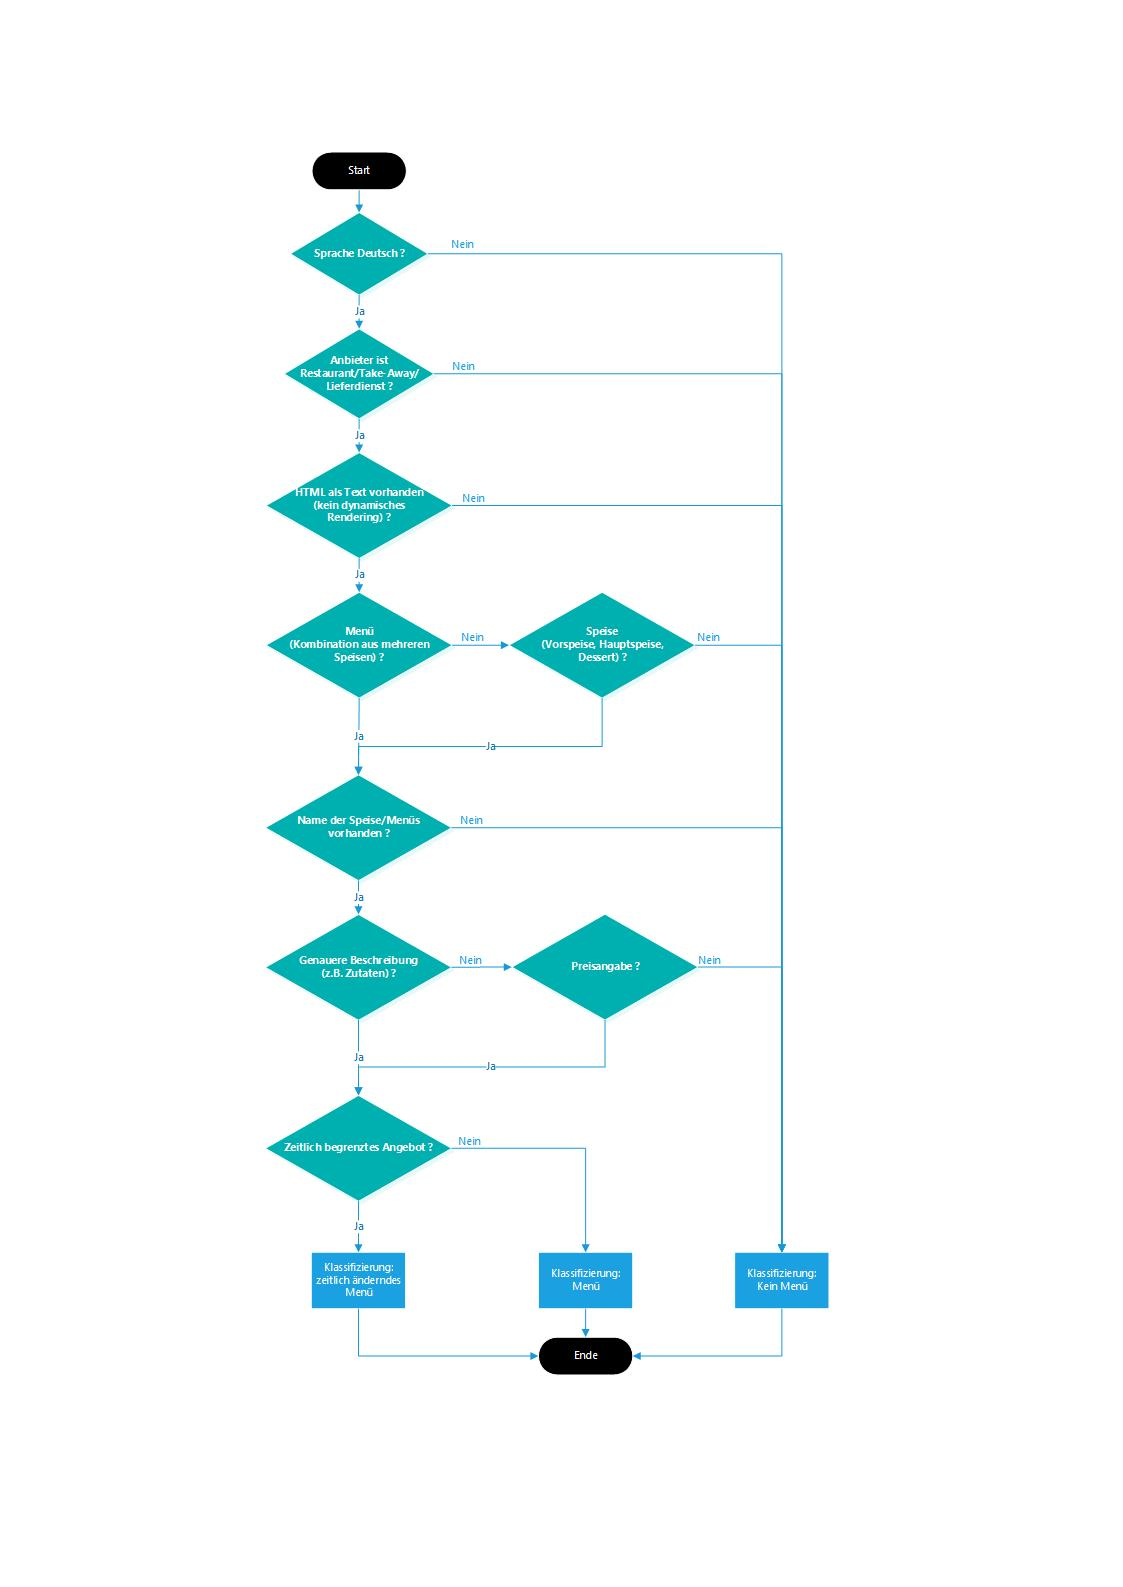
\includegraphics[width=1\columnwidth,keepaspectratio]{img/man-classification-tree.jpg}
\end{figure}
Obwohl bereits beim Webcrawler eine Spracherkennung eingesetzt wurde, damit nur als deutsch erkannte Webpages gespeichert werden, wurde bei der manuellen Klassifikation nochmals darauf geachtet, dass die Webpage in deutsch verfasst wurde.
Dabei ist anzumerken, dass gewisse Begriffe, vor allem für Speisebezeichnungen, auch fremdsprachig sein dürfen, da Speisebezeichnungen je nach Küche international ausgelegt sind.
Der Anbieter muss zwingend ein Restaurant, Take-Away oder Lieferdienst sein.
Der Inhalt muss als statisch verfügbar sein, da der Webcrawler nicht mit dynamisch gerenderten Websites umgehen kann.
Der Name der Speise und eine genauere Beschreibung oder der Preis muss vorhanden sein.
Danach folgt die Unterscheidung zwischen zeitlich begrenzten und unbegrenzten Angeboten, welche zur Kategorisierung führt.

\section{Seed}
Das Seed wurde aus den folgenden zwei Quellen zusammengestellt:
\begin{itemize}
	\item OpenStreetMap
	\item Lunch-Check
\end{itemize}
Daraus ist ein Seed entstanden, welches 5870 Einträge von Restaurant-URLs enthält.
Dabei wurden mehrere Einträge entfernt, aus den nun aufgeführten Gründen:
\begin{itemize}
	\item Die Website enthält mehr als 300 Webpages
	\item Die Website ist offensichtlich keine Restaurant-Website
\end{itemize}

